\documentclass{article}

\usepackage{geometry}
\usepackage{booktabs}
\usepackage{graphicx}

\geometry{margin=1in}
\setlength{\parindent}{0em}
\setlength{\parskip}{1em}

\begin{document}

\section{Introduction}

This is a progress report on the project of using BioBERT, a BERT language model pretrained on biomedical texts, to
detect relation between interesting biomedical entities found in ACS articles.

\section{Project Goals} 

This project has two goals. The first goal is to implement the BioBERT in a more recent deep learning framework for
easier maintainance and future-proving. We choose to reimplement the original version, which was in Tensorflow
1.15.2, with hugginface's transformers framework because of its support for both Tensorflow and PyTorch backends,
frequent updates, and rich functionalities.

The second goal is to fine-tune BioBERT, adapting it to the specific task of relation extraction. Because there
aren't any labeled relation extraction samples on the ACS articles, and using human annotator to create labeled
dataset on the entire set of ACS articles is currently beyond our resource constraints, We decide to fine-tune
BioBERT on the ChemProt dataset which contains samples of chemical-gene relationships. Then, the fine-tuned model is
applied to ACS Articles to detect chemical-gene relationships between biomedical entities.

\subsection{Implementation Details}

The model is implemented using hugginface's transoformers framework with PyTorch as the backend. Starting with
BERT-base cased model, we attached two fully connected linear units with tanh activation. A dropout unit with dropout
probability $p=0.1$ is inserted between the first and the second linear units.

\subsection{Fine-tuning BioBERT}

We start with BioBERT pretrained on PubMed and PMC texts. The model is fine-tuned on ChemProt dataset. During the
fine-tuning stage, the model starts training with a learning rate of 5e-6 and the learning is gradually decreasing
throughout the fine-tuning. Validation sets are used for every 1000 steps for early stopping and to prevent
overfitting on the training dataset. The network optimizer is the Adam optimizer with weights decay factor set to
0.01 and betas set to (0.9, 0.999).

\subsection{Detecting Relations in ACS Articles}

After the BioBERT is fine-tuned on ChemProt, it is run on ACS articles for entity relation extraction. The entities
inside ACS articles are detected by NER models in the upstream task.

\subsection{Results}

\begin{table}[ht]
\centering
\caption{Tensorflow Implmentation vs. Pytorch Implementation}
\label{tab:score-cmp}
\begin{tabular}{| c | c c | c c | c c |}
\toprule
Class & \multicolumn{2}{c}{Precision} & \multicolumn{2}{|c|}{Recall} & \multicolumn{2}{c|}{F1} \\
& Tensorflow & PyTorch & Tensorflow & PyTorch & Tensorflow & PyTorch \\
\midrule
Upregulator     & 0.7221    & 0.7307    & 0.7182    & 0.7400    & 0.7201    & 0.7357 \\
DownRegulator   & 0.8362    & 0.8124    & 0.8355    & 0.8272    & 0.8358    & 0.8197 \\
CPR-5           & 0.8140    & 0.8673    & 0.9052    & 0.8448    & 0.8571    & 0.8599 \\
CPR-6           & 0.7415    & 0.7755    & 0.7638    & 0.7638    & 0.7525    & 0.7696 \\
Substrate       & 0.6790    & 0.7174    & 0.6849    & 0.6499    & 0.6819    & 0.6820 \\
NoRelation      & 0.9509    & 0.9477    & 0.9490    & 0.9499    & 0.9499    & 0.9488 \\
\midrule
Weighted        & 0.9142    & 0.9125    & 0.9140    & 0.9130    & 0.9141    & 0.9127 \\
\bottomrule
\end{tabular}
\end{table}

\begin{figure}[ht]
\centering
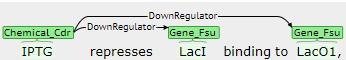
\includegraphics{brat1}
\caption{BioBERT detecting downregualor relation}
\label{fig:brat1}
\end{figure}

\begin{figure}[ht]
\centering
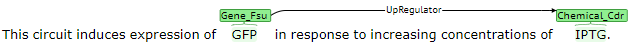
\includegraphics{brat2}
\caption{BioBERT detecting upregulator relation}
\label{fig:brat2}
\end{figure}

In table \ref{tab:score-cmp}, we are confident that the PyTorch implementation are very close to the original one
because of the similar scores. After verifying the implementation, we run prediction task on the ACS article.
Relation detected by the model are postprocessed into BRAT format and uploaded to a BRAT server, which helped us to
visualize the result (figure \ref{fig:brat1}, figure \ref{fig:brat2}).

\end{document}
